\chapter{Introduction}

\label{chapter:introduction}

In this chapter, we introduce this thesis by presenting its motivation,
describing our research questions and providing an overview of the thesis
structure.

\section{Motivation and objective}

There is a recent trend of increasingly complex deep learning models achieving
state-of-the-art performance on \ac{ml} and \ac{nlp} tasks, as shown in Figure
\ref{fig:nlp_progress}. To address emerging concerns such as security risks and
inductive biases, several studies argue for focused research into \ac{xai}
\citep{doran2017does,townsend2019extracting,danilevsky2020survey,arrieta2020explainable}.
Of these studies, \citet{arrieta2020explainable} provide an extensive overview
of \ac{xai} and related concepts based on a thorough literature review of
$\sim$400 \ac{xai} research contributions published to date. In particular,
\citet{arrieta2020explainable} explore and classify a variety of \ac{ml} models
into transparent and black-box categories depending on their degrees of
transparency. Furthermore, they explore taxonomies of post-hoc explainability
techniques aimed at effectively explaining black-box models. Notable
explainability techniques used in recent research include local explanations,
feature relevance and explanations by simplification.

Through our own survey of recent literature on explainability techniques in
\ac{nlp}, we came across several interesting studies employing the three
aforementioned post-hoc explainability techniques to better explain deep neural networks
\citep{schwartz2018sopa,peng2018rational,suresh-etal-2019-distilling,wang2019state,jiang2020cold}.
Of these studies, we draw inspiration from \citet{schwartz2018sopa} who
developed the novel hybridized \ac{rnn}, \ac{cnn} and weighted finite-state
\ac{sopa} model architecture with a special focus in model explainability. While
the \ac{sopa} model functions well, we find its explainability techniques to be
localized and indirect despite its neural architecture being suited for the
globalized and direct explanations by simplification explainability technique.
The main objective of this thesis is to address these limitations and to propose
a modified model, \textbf{\ac{spp}}, which could allow for effective explanations
by simplification. To facilitate this objective, we study both the performance and
explanations by simplification of the modified \ac{spp} model on the recently
released \ac{fmtod} data set from \citet{schuster-etal-2019-cross-lingual};
focusing on the English-language intent classification task.

\begin{figure}[t!]
  \centering
  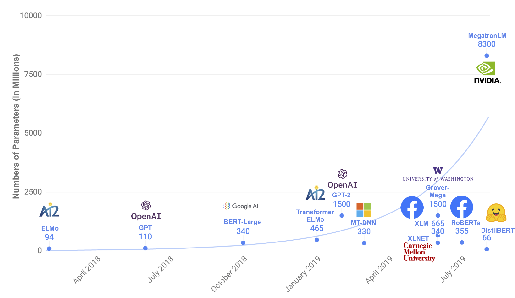
\includegraphics[width=13cm]{pdfs/borrowed/nlp_sota_model_size_progress.pdf}
  \caption{Parameter counts of recently released pre-trained language models
    which showed competitive or state-of-the-art performance when fine-tuned
    over a range of NLP tasks; figure taken from \citet{sanh2019distilbert}}
  \label{fig:nlp_progress}
\end{figure}

\section{Research questions}

\label{section:rq}

To guide us in addressing our objective, we aim to answer the following three
research questions:

\begin{enumerate}
  \item Does \ac{spp} provide competitive\footnote{We define
    competitive performance as the scenario where a mean performance metric on a
    certain task falls within the range obtained from other recent studies on
    the same task} performance on the \ac{fmtod} English language intent classification task?
  \item To what extent does \ac{spp} contribute to effective explanations by
  simplification on the \ac{fmtod} English language intent classification task?
  \item What interesting and relevant explanations can \ac{spp} provide on the
  \ac{fmtod} English language intent classification task?
\end{enumerate}

\section{Thesis structure}

We now summarize the contents and structure of this thesis.

\begin{description}[align=left]
  \item [Chapter \ref{chapter:introduction}:] Introduce this thesis, its
  contents and our research questions.
  \item [Chapter \ref{chapter:background}:] Describe the background concepts
  utilized in this thesis.
  \item [Chapter \ref{chapter:methodologies}:] Describe the \ac{fmtod} data set and
  methodologies pursued in this thesis.
  \item [Chapter \ref{chapter:results}:] Describe the results obtained from our
  methodologies.
  \item [Chapter \ref{chapter:discussion}:] Interpret the results and discuss their
  implications.
  \item [Chapter \ref{chapter:conclusions}:] Summarize the findings
  of this thesis.
  \item [Chapter \ref{chapter:further_work}:] Describe future work to expand on
  our research questions.
\end{description}

% LocalWords:  explainability pre NLP

%%% Local Variables: 
%%% mode: latex
%%% TeX-master: "main"
%%% End: